\documentclass{a4beamer}
%% Lectures - common definitions

\usextensions{tikz}
\usetikzlibrary{shapes.multipart,shapes.callouts,shapes.geometric}
\input{fix-callouts.inc} % Fixes absolute positioning of rectangle callouts

\newif\ifbigpages \bigpagesfalse
\ifdim\paperwidth >20cm
	\bigpagestrue
\fi

\tikzset{%
	note/.style={rectangle callout,draw=none,callout pointer width=1em,%
		align=flush left,font=\footnotesize,inner sep=0.5em,%
		fill=blue!15,fill opacity=0.95,text opacity=1.0,callout absolute pointer=#1},
	node distance=2em and 2.75em
}
\ifbigpages
	% Scale all arrow tips by the factor of 2.5
	\let\old@pgf@arrow@call=\pgf@arrow@call
	\def\pgf@arrow@call#1{%
		\@tempdima=\pgflinewidth%
		\pgfsetlinewidth{2.5\pgflinewidth}%
		\old@pgf@arrow@call{#1}%
		\pgfsetlinewidth{\@tempdima}%
	}
	\def\pgfarrowsleftextend#1{\pgfmathsetlength{\pgf@xa}{1.5*#1}}
	\def\pgfarrowsrightextend#1{\pgfmathsetlength{\pgf@xb}{1.5*#1}}
\fi

%% Load listings package
\usepackage{listings}

%% Are we inside a comment?
\newif\iflstcomment \lstcommentfalse

\lstset{%
	tabsize=4,
	showstringspaces=false,
	basicstyle=\linespread{1.25}\ttfamily\small,
	keywordstyle=\bfseries,
	commentstyle=\lstcommentstyle,
	numbers=left,
	numberstyle=\footnotesize\color{gray},
	xleftmargin=2.5em,
	extendedchars=true,
	escapechar=\$,
	escapebegin=\iflstcomment\begingroup\lstcommentstyle\fi,
	escapeend=\iflstcomment\endgroup\fi
}

\def\lstcommentstyle{\color{gray}}

\lst@AddToHook{AfterBeginComment}{\global\lstcommenttrue}
\let\orig@lst@EndComment=\lst@EndComment
\def\lst@EndComment{\global\lstcommentfalse\orig@lst@EndComment}
\lst@AddToHookAtTop{EOL}{%
	\lst@ifLmode\global\lstcommentfalse\fi% XXX Sloppy way to determine comment end
}

%% Python with docstrings treated as comments
\lstdefinelanguage[doc]{python}[]{python}{%
	deletestring=[s]{"""}{"""},%
	morecomment=[s]{"""}{"""}%
}%

%% JavaScript language
\lstdefinelanguage{javascript}%
	{morekeywords={break,case,catch,%
		const,constructor,continue,default,do,else,false,%
		finally,for,function,if,in,instanceof,%
		new,null,prototype,%
		return,switch,this,throw,%
		true,try,typeof,var,while},%
	sensitive,%
	morecomment=[l]//,%
	morecomment=[s]{/*}{*/},%
	morestring=[b]",%
	morestring=[b]',%
}[keywords,comments,strings]%

%% C# language (4.0?)
\lstdefinelanguage{csharp}%
	{morekeywords={abstract,as,%
		base,bool,byte,case,catch,char,%
		checked,class,const,continue,%
		decimal,default,delegate,do,double,%
		else,enum,event,explicit,extern,%
		false,finally,fixed,float,for,foreach,%
		goto,if,implicit,in,int,interface,%
		internal,is,lock,long,%
		namespace,new,null,object,operator,out,%
		override,params,private,protected,public,%
		readonly,ref,return,sbyte,sealed,%
		short,sizeof,stackalloc,static,string,%
		struct,switch,this,throw,true,try,%
		typeof,uint,ulong,unchecked,unsafe,ushort,%
		using,virtual,void,volatile,while%
	},%
	sensitive,%
	morecomment=[l]//,%
	morecomment=[s]{/*}{*/},%
	morestring=[b]",%
	morestring=[b]',%
}[keywords,comments,strings]%

%% Translation for fact environment
\deftranslation[to=russian]{Fact}{Наблюдение}

%% Inline code snippets
\def\code#1{\texttt{#1}}
\def\codekw#1{\code{\textbf{#1}}}

\def\quoteauthor#1{\par\footnotesize\upshape\hfill—~#1}

%% English term
\def\engterm#1{(англ. \textit{#1})}
%% Term with explanation below (to be used in diagrams)
\def\termwithexpl#1#2{#1\strut{}\\\small\color{gray}(\textit{#2})\strut{}}
%% External link
\def\extlink#1#2{\href{#1}{\color[rgb]{0.7,0.7,1.0}\dashbar{#2}}}
%% Internal link
\def\inlink#1#2{\hyperlink{#1}{\color[rgb]{0.7,0.7,1.0}\dashbar{#2}}}
%% Explanation for a list item
\def\itemexpl#1{\begingroup\small\vspace{0.75ex}#1\par\endgroup}



\usepackage{multicol}
\usetikzlibrary{shapes.misc}


\lecturetitle{Программная инженерия. Лекция №23 — Управление качеством ПО}
\title[Качество]{Управление качеством ПО}
\author{Алексей Островский}
\institute{\small{Физико-технический учебно-научный центр НАН Украины}\vspace{2ex}}
\date{7 мая 2015 г.}

\begin{document}
	\frame{\titlepage}

	\section{Качество}

	\subsection{Определение}

	\frame{
		\frametitle{Качество ПО}

		\begin{Definition}
			\textbf{Качество} — две взаимосвязанных характеристики разрабатываемого программного продукта:
			\begin{itemize}
				\item
				мера, в которой ПО соответствует \emph{функциональным требованиям}, заданным планом разработки 
				и~прочими документами спецификации (функциональное качество);

				\item
				уровень поддержки \emph{нефункциональных требований}: надежности, производительности, … (структурное качество).
			\end{itemize}
		\end{Definition}

		\vspace{1ex}
		\textbf{Поддержание качества:}
		\begin{itemize}
			\item
			функциональное качество — с помощью тестирования;
			\item
			структурное качество — с помощью соответствия стандартам и статического анализа кода.
		\end{itemize}
	}

	\subsection{Оценка}

	\frame{
		\frametitle{Оценка качества}

		\begin{itemize}
			\item
			Были ли в процессе разработки учтены \textbf{стандарты кодирования и~документирования} ПО?

			\vspace{0.5ex}
			\item
			Были ли проведены достаточное \textbf{тестирование и / или верификация} ПО?

			\vspace{0.5ex}
			\item
			Достаточно ли \textbf{надежен} программный продукт?

			\vspace{0.5ex}
			\item
			Удовлетворительна ли \textbf{скорость работы и время отклика} ПО?

			\vspace{0.5ex}
			\item
			Обладает ли ПО достаточно понятным \textbf{пользовательским интерфейсом}?

			\vspace{0.5ex}
			\item
			Является ли программная система \textbf{модульной}? В~какой степени она поддерживает \textbf{сопровождение}, 
			в~частности, внесение изменений?
		\end{itemize}
	}

	\subsection{Управление качеством}

	\frame{
		\frametitle{Управление качеством}

		\begin{Definition}
			\textbf{Управление качеством ПО} \engterm{software quality management} — деятельность, 
			направленная на~поддержание уровня качества программной системы.
		\end{Definition}

		\vspace{1ex}
		\textbf{Составляющие процессы:}
		\begin{itemize}
			\item
			\textbf{обеспечение качества} \engterm{quality assurance, QA} — определение стандартов 
			и~регламентирующих документов для~производства, проверки и~оценки программных продуктов;

			\item
			\textbf{планирование качества} \engterm{software quality plan} — применение стандартов 
			и~инструментов для~поддержания качества в~конкретном программном проекте;

			\item
			\textbf{контроль качества} \engterm{software quality control} — соблюдение планирования качества 
			и~обеспечения качества во~время разработки.
		\end{itemize}
	}

	\frame{
		\frametitle{Планирование качества}

		\textbf{План обеспечения качества:}
		\begin{itemize}
			\item
			желаемые характеристики качества ПО;
			\item
			методы оценки и достижения характеристик качества.
		\end{itemize}

		\vspace{1ex}
		\textbf{Примерное содержание:}
		\begin{itemize}
			\item описание продукта, рынка сбыта, ожидаемых характеристик качества;
			\item планы разработки, крайние даты выпуска;
			\item описание процессов разработки и используемых стандартов;
			\item описание и обоснование важнейших характеристик качества;
			\item ключевые риски при разработке, методы их минимизации.
		\end{itemize}
	}

	\section{Стандарты}

	\frame{
		\frametitle{Стандарты}

		\begin{Definition}
			\textbf{Стандарты ПО} \engterm{software standard} — документы, регламентирующие определенные аспекты 
			производства программной системы.
		\end{Definition}

		\vspace{1ex}
		\textbf{Категории:}
		\begin{itemize}
			\item
			\textbf{стандарты продуктов} \engterm{product standards} — стандарты, 
			касающиеся конечных или~промежуточных артефактов разработки: 
			структура документов, стандарты оформления кода, содержание комментариев, …

			\item
			\textbf{стандарты процессов} \engterm{process standards} — описание процессов при~разработке~ПО: 
			процессы спецификации, проектирования и~тестирования, используемые инструменты, …
		\end{itemize}
	}

	\frame{
		\frametitle{Примеры стандартов}

		\textbf{Стандарты продуктов:} 
		\begin{itemize}
			\item структура документа спецификации; 
			\item формат документирования методов;
			\item стандарт оформления кода;
			\item формат плана проекта;
			\item форма запроса на изменение.
		\end{itemize}

		\vspace{1ex}
		\textbf{Стандарты процессов:}
		\begin{itemize}
			\item порядок проведения рецензии на дизайн;
			\item процесс выпуска версии ПО;
			\item процесс фиксации изменений;
			\item процесс внедрения плана проекта;
			\item процесс проведения тестирования.
		\end{itemize}
	}

	\subsection{ISO 9001}

	\frame{
		\frametitle{Стандарт ISO 9001}

		Стандарт ISO 9001 определяет \textbf{категории процессов производства} произвольных продуктов. 
		Соответствие стандарту — определение отношений между конкретными процессами разработки ПО и~категориями.

		\vspace{1ex}
		\textbf{Процессы поставки продукта:}
		\begin{itemize}
			\item приобретение бизнеса \engterm{business acquisition};
			\item проектирование и разработка;
			\item тестирование;
			\item производство и поставка \engterm{production and delivery};
			\item обслуживание и поддержка.
		\end{itemize}

		\vspace{1ex}
		\textbf{Вспомогательные процессы:}
		\ifbigpages\vspace{-1ex}\else\vspace{-2ex}\fi
		\begin{multicols}{2}
			\begin{itemize}
				\item управление бизнесом;
				\item управление поставками;
				\item управление ресурсами;
				\item управление конфигурацией.
			\end{itemize}
		\end{multicols}
	}

	\frame{
		\frametitle{Стандарт ISO 9001}

		\begin{figure}
			{\small\begin{tikz*}[%
	every node/.style={rectangle,draw,align=center,minimum height=3em},
	label/.style={draw=none,font=\footnotesize\itshape,minimum height=0pt},
	action/.style={rounded rectangle}
]
	\node(models) {Модели качества \\ ISO 9001};
	\node(manual) [below=4em of models] {Руководство качества \\ организации};
	\node(plan2) [below=4em of manual] {План качества \\ проекта 2};
	\node(plan1) [left=of plan2] {План качества \\ проекта 1};
	\node(plan3) [right=of plan2] {План качества \\ проекта 3};
	\node(management) [right=of plan3,action] {Управление качеством \\ проекта};
	\node(process) at (management.center |- manual.center) [action] {Процессы поддержки \\ качества};

	\draw[->] (models) -- node[label,right] {реализованы в} (manual);
	\draw[->] (manual) -- (plan1);
	\draw[->] (manual) -- (plan3);
	\draw[->] (manual) -- node[label,fill=white] {используется для разработки} (plan2);
	\draw[->] (manual) -- node[label,above] {документирует} (process);
	\draw[->] (process) -- node[label,left] {реализованы в} (management);

	\node(_tmp) [coordinate,below=2em of management.south] {};
	\draw (plan1.south) |- node[label,below,pos=0.75] {поддерживают} (_tmp);
	\draw[->] (_tmp) -- (management.south);
	\draw (plan2.south) -- (plan2.south |- _tmp);
	\draw (plan3.south) -- (plan3.south |- _tmp);
\end{tikz*}
}
			\caption{Использование стандарта ISO 9001 при разработке ПО}
		\end{figure}
	}

	\section[Инспекции]{Обзоры и инспекции}

	\frame{
		\frametitle{Обзоры и инспекции}

		\begin{Definition}
			\textbf{Обзоры} \engterm{review} и \textbf{инспекции} \engterm{inspection} — процессы обеспечения качества, 
			предназначенные для~оценки качества артефактов разработки~ПО (программ, документации, диаграмм проектирования и~т.\,п.).
		\end{Definition}

		\vspace{2ex}
		\textbf{Обзор} — формальный подход: команда разработчиков, проверка на~соответствие установленным стандартам.

		\vspace{1ex}
		\textbf{Инспекция} — менее формальный подход: кооперация между~разработчиками, поиск ошибок и~пропусков.
	}

	\subsection{Области проверки кода}

	\frame{
		\frametitle{Области проверки кода}

		\begin{itemize}
			\item
			\textbf{Дефекты данных:}
			\begin{itemize}
				\item инициализация переменных перед использованием; 
				\item отсутствие «магических» констант; 
				\item индексация элементов массивов / списков; 
				\item потенциальные случаи переполнения буфера.
			\end{itemize}

			\vspace{1ex}
			\item
			\textbf{Дефекты выполнения:} 
			\begin{itemize}
				\item проверка условий ветвления; 
				\item конечность циклов; 
				\item корректность блоков операций; 
				\item полнота вариантов и наличие \textbf{break} в операторе \textbf{switch} / \textbf{case}.
			\end{itemize}

			\vspace{1ex}
			\item
			\textbf{Дефекты ввода/вывода:} 
			\begin{itemize}
				\item использование всех входных переменных; 
				\item присвоение выходных переменных.
			\end{itemize}
		\end{itemize}
	}

	\frame{
		\frametitle{Области проверки кода}

		\begin{itemize}
			\item
			\textbf{Дефекты интерфейсов:}
			\begin{itemize}
				\item корректное количество и порядок аргументов при вызове функций / методов; 
				\item соответствие ожидаемых и фактических типов аргументов; 
				\item идентичность структуры разделяемой памяти.
			\end{itemize}

			\vspace{1ex}
			\item
			\textbf{Дефекты работы с памятью:} 
			\begin{itemize}
				\item корректность работы со связанными объектами (изменение всех требуемых ссылок); 
				\item корректность выделения / освобождения памяти.
			\end{itemize}

			\vspace{1ex}
			\item
			\textbf{Дефекты обработки исключений:} 
			\begin{itemize}
				\item полнота проверок возникновения исключительных ситуаций.
			\end{itemize}
		\end{itemize}
	}

	\subsection{Инспекции в гибкой методологии}

	\frame{
		\frametitle{Инспекции в гибкой методологии}

		\begin{figure}
			\ifbigpages
				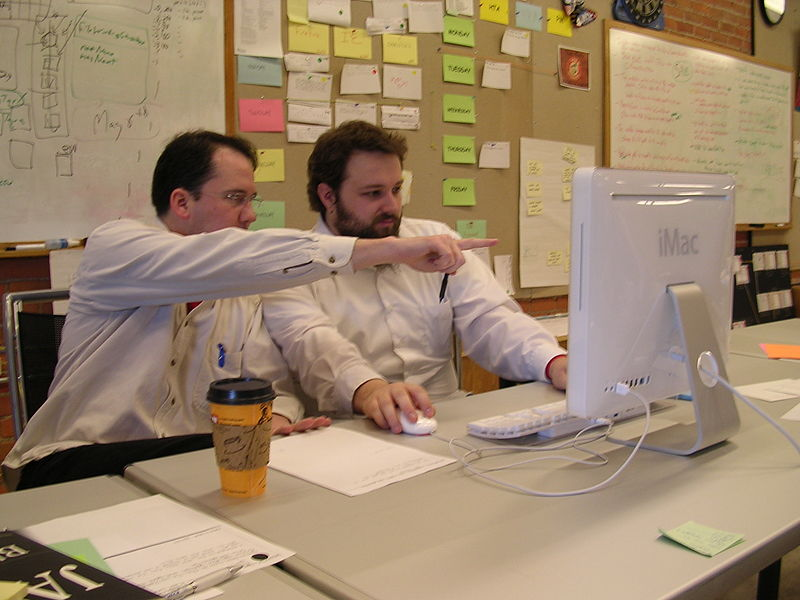
\includegraphics[scale=2.0]{fig-pair-programming.jpg}
			\else
				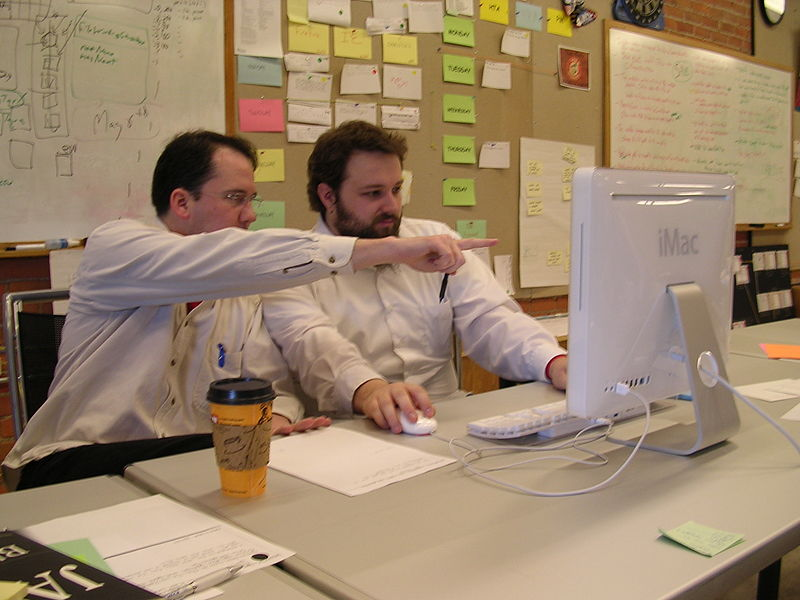
\includegraphics[scale=1.0]{fig-pair-programming.jpg}
			\fi
			\caption{В гибкой методологии разработки наряду или~вместо обзоров и~инспекций 
				используется парное программирование \engterm{pair programming}.}
		\end{figure}
	}

	\frame{
		\frametitle{Парное программирование}

		\begin{Definition}
			\textbf{Парное программирование} \engterm{pair programming} — способ разработки~ПО, 
			при~котором код, написанный первым программистом, немедленно проверяется вторым программистом; 
			альтернатива формальным инспекциям в гибкой методологии разработки.
		\end{Definition}

		\vspace{1.5ex}
		\textbf{Достоинства:} более глубокое понимание кода $\Rightarrow$ обнаружение большего числа дефектов.

		\vspace{1ex}
		\textbf{Недостатки:} 
		\begin{itemize}
			\item повышенный шанс непонимания требований; 
			\item пропуск ошибок из-за высокого темпа разработки; 
			\item необъективность инспектора.
		\end{itemize}
	}

	\section{Измерение ПО}

	\frame{
		\frametitle{Измерение качества}

		\begin{Definition}
			\textbf{Измерение ПО} — описание аспектов программной системы, отдельных ее~компонентов 
			или~процессов разработки с~помощью математического аппарата.
		\end{Definition}

		\vspace{1ex}
		\textbf{Цели измерения ПО:}
		\begin{itemize}
			\item
			замена дорогостоящих процессов обеспечения качества (напр., обзоров);
			\item
			идентификация компонентов ПО, подлежащих изменению.
		\end{itemize}

		\vspace{1ex}
		\textbf{NB.} На сегодняшний день не существует полностью автоматизированных инструментов оценки качества 
		на~основе измерений; результаты измерений анализируются человеком.
	}

	\subsection{Модели}

	\frame{
		\frametitle{Модели качества}

		\begin{Definition}
			\textbf{Модель качества ПО} — математическая модель, позволяющая оценивать различные характеристики качества 
			на~основе анализа программы.
		\end{Definition}

		\vspace{1ex}
		\textbf{Уровни модели качества ПО:}
		\begin{enumerate}
			\item
			определение основных и вторичных характеристик качества~ПО 
			(надежность, удобство использования, …);
			\item
			определение измеряемых метрик для~каждой характеристики 
			(напр., число ошибок на~строку кода);
			\item
			измерение характеристик качества с помощью метрик в~статике (анализ структуры программы) 
			и~динамике (выполнение программы);
			\item
			агрегация метрик, выделение наиболее важных характеристик качества.
		\end{enumerate}
	}

	\subsection{Характеристики}

	\frame{
		\frametitle{Характеристики качества}

		\begin{figure}
			\def\submember#1{\small\color{gray}#1\strut{}}
\begin{tikz*}[%
	every node/.style={draw,align=center},
	attr/.style={rectangle split,rectangle split parts=2,minimum width=10.5em}
]
	\node(attr) [minimum width=35em,font=\large\bfseries] {Характеристики ПО};

	\node(functionality) [attr,above=of attr] {%
		\textbf{Функциональность} 
		\nodepart{two}
		\submember{полнота функций} \\ 
		\submember{точность} \\ 
		\submember{интероперабельность} \\ 
		\submember{защищенность}
	};
	\node(reliability) [attr,left=of functionality.south west,anchor=south east] {%
		\textbf{Надежность} 
		\nodepart{two}
		\submember{зрелость} \\ 
		\submember{отказоустойчивость} \\ 
		\submember{возобновляемость}
	};
	\node(efficiency) [attr,right=of functionality.south east,anchor=south west] {%
		\textbf{Эффективность} 
		\nodepart{two}
		\submember{реактивность} \\ 
		\submember{ресурсоемкость} \\ 
		\submember{емкость}
	};


	\node(portability) [attr,below=of attr] {%
		\textbf{Переносимость} 
		\nodepart{two}
		\submember{простота адаптации} \\
		\submember{простота установки} \\
		\submember{совместимость} \\
		\submember{заменяемость}
	};
	\node(usability) [attr,right=of portability.north east,anchor=north west] {%
		\textbf{Удобство} \\ \textbf{использования} 
		\nodepart{two}
		\submember{понятность} \\ 
		\submember{обучаемость} \\ 
		\submember{работоспособность} \\ 
		\submember{привлекательность}
	};
	\node(maintainability) [attr,left=of portability.north west,anchor=north east] {%
		\textbf{Удобство} \\ \textbf{сопровождения} 
		\nodepart{two}
		\submember{простота анализа} \\
		\submember{простота изменений} \\
		\submember{стабильность} \\
		\submember{простота тестирования}
	};

	\draw[->] (attr) -- (functionality);
	\draw[->] (attr.north -| reliability.south) -- (reliability.south);
	\draw[->] (attr.north -| efficiency.south) -- (efficiency.south);
	\draw[->] (attr) -- (portability);
	\draw[->] (attr.south -| usability.north) -- (usability.north);
	\draw[->] (attr.south -| maintainability.north) -- (maintainability.north);
\end{tikz*}

			\caption{Основные и вторичные характеристики качества ПО согласно стандарту ISO 9126}
		\end{figure}
	}

	\frame{
		\frametitle{Функциональность}

		\begin{Definition}
			\textbf{Функциональность} \engterm{functionality} — группа характеристик, оценивающих способность программной системы 
			выполнять функции, заданные с~помощью документов спецификации или~неявно.
		\end{Definition}

		\vspace{1ex}
		\textbf{Составляющие:}
		\begin{itemize}
			\item
			\textbf{функциональная полнота} \engterm{suitability} — достаточность основных функций~ПО 
			для~решения задач, определяемых функциональными требованиями;

			\item
			\textbf{точность} \engterm{accuracy} — достижение корректных результатов 
			для~всех наборов входных данных;

			\item
			\textbf{интероперабельность} \engterm{interoperability} — возможность взаимодействия с~системой 
			посредством внешних интерфейсов (напр., средствами~ОС или~с~помощью сети);

			\item
			\textbf{защищенность} \engterm{security} — способность предотвращать несанкционированный доступ 
			к~функциям программы и~данным.
		\end{itemize}
	}

	\frame{
		\frametitle{Надежность}

		\begin{Definition}
			\textbf{Надежность} \engterm{reliability} — группа характеристик, определяющих способность программной системы 
			выполнять свои функции в~течение определенного периода времени.
		\end{Definition}

		{\small\textbf{NB.} Надежность определяется для программной системы и~не~зависит от~оборудования 
		или~мнения пользователей.}

		\vspace{1ex}
		\textbf{Составляющие:}
		\begin{itemize}
			\item
			\textbf{зрелость} \engterm{maturity} — способность ПО функционировать без~отказов 
			в~нормальных условиях;

			\item
			\textbf{отказоустойчивость} \engterm{fault tolerance} — способность ПО функционировать в~аномальных условиях 
			(сбой аппаратуры, ошибки в~данных и~интерфейсах, некорректные действия пользователя, …);

			\item
			\textbf{возобновляемость} \engterm{recoverability} — способность перезапуска 
			для~повторного использования и~восстановления данных после~отказов~ПО.
		\end{itemize}
	}

	\frame{
		\frametitle{Удобство использования}

		\begin{Definition}
			\textbf{Удобство использования} \engterm{usability} — группа характеристик, 
			связанных с~эргономичностью программного продукта; 
			характеристики, влияющие на~выбор~ПО определенной группой пользователей для~решения конкретных задач.
		\end{Definition}

		\vspace{1ex}
		\textbf{Составляющие:}
		\begin{itemize}
			\item
			\textbf{понимаемость} \engterm{undestandability} — оценка усилий, затраченных на~выяснение логических концепций 
			и~условий применения~ПО;

			\item
			\textbf{обучаемость} \engterm{learnability} — оценка усилий, затраченных на определение принципов функционирования~ПО 
			с~помощью документации, правил, диагностики и~т.\,п.;

			\item
			\textbf{работоспособность} \engterm{operability} — простота работы и~управления системой;

			\item
			\textbf{привлекательность} \engterm{attractiveness} — соответствие пользовательского интерфейса программы 
			ожиданиям пользователей.
		\end{itemize}
	}

	\frame{
		\frametitle{Эффективность}

		\begin{Definition}
			\textbf{Эффективность} \engterm{efficiency} — группа характеристик, определяющих производительность системы 
			относительно потребляемых ресурсов при~заданных условиях.
		\end{Definition}

		\vspace{1ex}
		\textbf{Составляющие:}
		\begin{itemize}
			\item
			\textbf{реактивность} \engterm{time behaviour} — оценка времени отклика, 
			обработки и~выполнения функций~ПО;

			\item
			\textbf{использование ресурсов} \engterm{resource utilization} — соответствие использования 
			различных видов ресурсов заданным требованиям;

			\item
			\textbf{емкость} \engterm{capacity} — степень соответствия ограничений системы 
			(напр., максимальное количество пользователей в~произвольный момент времени) требованиям.
		\end{itemize}
	}

	\frame{
		\frametitle{Удобство сопровождения}

		\begin{Definition}
			\textbf{Удобство сопровождения} \engterm{maintainability} — множество характеристик, оценивающих усилия, 
			затрачиваемые на~эволюцию~ПО: устранение дефектов, совершенствование и~адаптацию.
		\end{Definition}

		\vspace{1ex}
		\textbf{Составляющие:}
		\begin{itemize}
			\item
			\textbf{простота анализа} \engterm{analyzability} — оценка усилий для~диагностики отказов~ПО 
			и~идентификации компонентов для~изменения;

			\item
			\textbf{простота изменений} \engterm{changeability} — степень, в~которой программная система 
			допускает модификацию без~внесения дефектов;

			\item
			\textbf{стабильность} \engterm{stability} — степень, в~которой программная система допускает 
			внесение изменений без~снижения качества существующих компонентов;

			\item
			\textbf{простота тестирования} \engterm{testability} — оценка усилий для~разработки критериев тестирования 
			и~набора тестов, с~помощью~которых можно подтвердить выполнение этих~критериев.
		\end{itemize}
	}

	\frame{
		\frametitle{Переносимость}

		\begin{Definition}
			\textbf{Переносимость} \engterm{portability} — множество характеристик, 
			оценивающих способность программной системы адаптироваться к~работе в~новом окружении.
		\end{Definition}

		\vspace{1ex}
		\textbf{Составляющие:}
		\begin{itemize}
			\item
			\textbf{адаптивность} \engterm{adaptability} — оценка усилий на~адаптацию к~другому оборудованию, 
			ПО или~другим компонентам окружения;

			\item
			\textbf{простота установки} \engterm{installability} — эффективность установки и~удаления 
			программной системы в~заданной среде;

			\item
			\textbf{сосуществование} \engterm{co-existence} — эффективность работы программной системы 
			при~разделении среды выполнения и~ее~ресурсов с~другим~ПО;

			\item
			\textbf{заменяемость} \engterm{replaceability} — эффективность замены аналогичного программного продукта 
			в~заданной среде выполнения.
		\end{itemize}
	}

	\subsection{Метрики качества}

	\frame{
		\frametitle{Метрики качества}

		\begin{Definition}
			\textbf{Метрика ПО} \engterm{software metric} — характеристика программной системы, 
			артефактов разработки (напр., системной документации) или~процессов разработки, 
			которую можно объективно измерить.
		\end{Definition}

		\vspace{1ex}
		\textbf{Примеры метрик:}
		\begin{itemize}
			\item количество строк кода;
			\item количество дефектов на строку кода;
			\item время выполнения программы;
			\item покрытие кода тестами \engterm{code coverage};
			\item \extlink{http://en.wikipedia.org/wiki/Cyclomatic_complexity}{цикломатическая сложность} \engterm{cyclomatic complexity}.
		\end{itemize}
	}

	\frame{
		\frametitle{Категории метрик ПО}

		\textbf{По объекту измерения:}
		\begin{itemize}
			\item
			метрики продукта, оценивающие характеристики ПО или артефактов производства (напр., документации);
			\item
			метрики процессов, оценивающие характеристики процессов разработки;
			\item
			метрики использования, оценивающие свойства ПО при~работе с~конечным пользователем.
		\end{itemize}

		\vspace{0.5ex}
		\textbf{По видимости:}
		\begin{itemize}
			\item
			внешние метрики, описывающие свойства~ПО, доступные для~конечного пользователя;
			\item
			внутренние метрики, описывающие свойства, доступные только~разработчикам.
		\end{itemize}

		\vspace{0.5ex}
		\textbf{По способу измерения:}
		\begin{itemize}
			\item
			динамические (требующие выполнения программы);
			\item
			статические, получаемые анализом проекта~ПО, кода или~документации.
		\end{itemize}
	}

	\frame{
		\frametitle{Метрики продукта}

		\textbf{Примеры общих метрик продукта:}
		\begin{itemize}
			\item
			\textbf{коэффициенты разветвления} \engterm{fan-in / fan-out} — количество функций, 
			вызывающих определенную функцию (fan-in); количество функций, которые вызывает определенная функция (fan-out);

			\item
			\textbf{размер кода} для отдельных функций / методов, классов, компонентов;

			\item
			\textbf{цикломатическая сложность} \engterm{cyclomatic complexity} — 
			количество линейно независимых маршрутов через граф потока управления программы;

			\item
			\textbf{длина идентификаторов} — средняя длина идентификаторов в~исходном коде 
			(локальные переменные, названия классов, методов, …);

			\item
			\textbf{глубина вложенных конструкций} — максимальное количество вложенных конструкций ветвления / цикла.
		\end{itemize}
	}

	\frame{
		\frametitle{Метрики продукта}

		\textbf{Примеры метрик продукта в ООП} [Chidamber, Kemerer, 1994]:
		\begin{itemize}
			\item
			\textbf{взвешенное количество методов} \engterm{weighted methods per class} — 
			сумма весов методов класса (вес~метода определяется его сложностью);

			\item
			\textbf{глубина дерева наследования} \engterm{depth of inheritance tree} — 
			количество уровней в~графе, представляющем отношение наследования;

			\item
			\textbf{число потомков} \engterm{number of children} — 
			среднее число непосредственных потомков для~класса;

			\item
			\textbf{связь между классами} \engterm{coupling between object classes} — мера, 
			в~которой методы одного класса используют методы другого класса;

			\item
			\textbf{реагирование} \engterm{response for a class} — количество методов, 
			которые могут быть вызваны при~обработке определенного сообщения.
		\end{itemize}
	}

	\subsection{Процесс измерения}

	\frame{
		\frametitle{Метрики и характеристики качества}

		\begin{figure}
			{\small\begin{tikz*}[%
	every node/.style={rectangle,draw,align=center,minimum height=3em,minimum width=10em},
	label/.style={draw=none,font=\bfseries}
]
	\node(tree) {Глубина дерева \\ наследования};
	\node(cycle) [below=of tree] {Цикломатическая \\ сложность};
	\node(size) [below=of cycle] {Размер программ};
	\node(error) [below=of size] {Число сообщений \\ об ошибках};
	\node(manual) [below=of error] {Размер руководства \\ по использованию};
	\node(metrics) [label,above=0pt of tree] {Метрики};

	\node(maint) [above left=1em and 25em of size.center,anchor=south] {Удобство \\ сопровождения};
	\node(port) [below left=1em and 25em of size.center,anchor=north] {Переносимость};
	\node(rely) [above=of maint] {Надежность};
	\node(use) [below=of port] {Удобство \\ использования};
	\node(attr) [label,left=25em of metrics.center,anchor=center] {Характеристики качества};

	\draw (rely.east) -- (cycle.west);
	\draw (rely.east) -- (size.west);
	\draw (rely.east) -- (error.west);

	\draw (maint.east) -- (tree.west);
	\draw (maint.east) -- (cycle.west);
	\draw (maint.east) -- (size.west);
	\draw (maint.east) -- (manual.west);

	\draw (use.east) -- (error.west);
	\draw (use.east) -- (manual.west);

	\draw (port.east) -- (tree.west);
	\draw (port.east) -- (size.west);
\end{tikz*}
}
			\caption{Связь метрик ПО с характеристиками качества}
		\end{figure}
	}

	\frame{
		\frametitle{Процесс измерения}

		\textbf{Этапы измерения ПО:}
		\begin{enumerate}
			\item
			Выбор необходимых измерений в соответствии с~заданной целью.
			\item
			Выбор компонентов, для которых производится измерение (напр., репрезентативная выборка 
			или~ключевые компоненты).
			\item
			Измерение характеристик компонентов с~помощью автоматических утилит.
			\item
			Идентификация аномальных измерений путем сравнения данных для~различных компонентов 
			и~с~результатами предыдущих измерений.
			\item
			Анализ аномальных компонентов в~соответствии с~замеренными данными.
		\end{enumerate}
	}

	\section{Заключение}

	\subsection{Выводы}
	
	\frame{
		\frametitle{Выводы}

		\begin{enumerate}
			\item
			Качество программного продукта означает его соответствие функциональным и~нефункциональным требованиям.

			\vspace{0.5ex}
			\item
			Управление качеством — отдельный аспект производства~ПО, включающий подбор стандартов, 
			разработку плана поддержки качества и~контролирование качества продуктов производства.

			\vspace{0.5ex}
			\item
			Контроль качества осуществляется с~помощью тестирования и~инспекций программ. 
			В~гибкой методологии инспекциям соответствуют неформальные методы контроля, 
			такие~как парное программирование.

			\vspace{0.5ex}
			\item
			Альтернативный способ оценки качества — измерение~ПО. 
			Измеримые метрики связаны с~характеристиками качества.
		\end{enumerate}
	}
	
	\subsection{Материалы}
	
	\frame{
		\frametitle{Материалы}
		
		\begin{thebibliography}{9}
			\bibitem[1]{1}
			Sommerville, Ian
			\newblock Software Engineering.
			\newblock {\footnotesize Pearson, 2011. — 790 p.}

			\bibitem[2]{2}
			Лавріщева К.\,М. 
			\newblock Програмна інженерія (підручник). 
			\newblock {\footnotesize К., 2008. — 319 с.}
		\end{thebibliography}
	}
	
	\frame{
		\frametitle{}
		
		\begin{center}
			\Huge Спасибо за внимание!
		\end{center}
	}

\end{document}

